\chapter{Numerical Double Integration}

In an earlier chapter, we gave an example of the multivariate normal distribution: the mass and shell diameter of a population of snails.

Starting with a table of measurements, we estimated that the mean vector $\mu$ was $\begin{bmatrix}4.25 \text{g} & 2.35 \text{cm}\end{bmatrix}$

Then we computed the covariance matrix:

\begin{equation*}
\mathbf{\Sigma} = \begin{bmatrix}
1.33 &  0.443 \\
0.443 & 0.416 \\
\end{bmatrix}
\end{equation*}

Plotting the data points, the mean, and the equal-density contours looked like this:

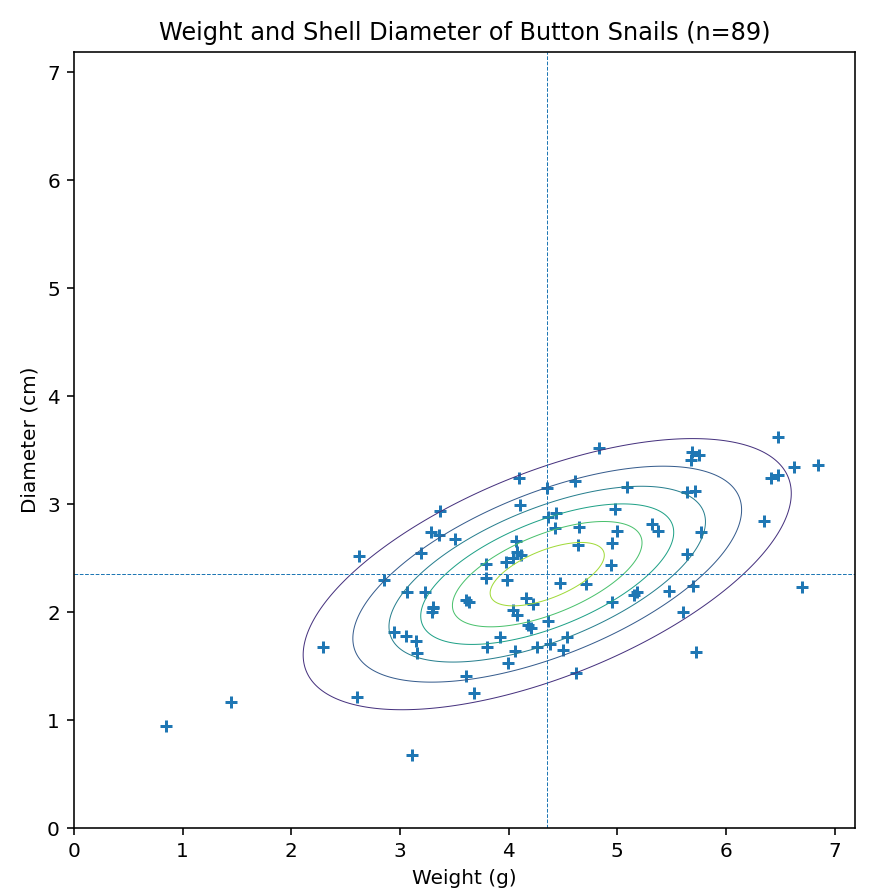
\includegraphics[width=0.55\textwidth]{contour.png}

We have a great formula for computing the probability density for any mass/diameter combination:

\begin{equation*}
p(\mathbf{x}) = \frac{1}{\sqrt{(2\pi)^d|\mathbf{\Sigma}|}}\exp\left(-\frac{1}{2}(\mathbf{x}-\boldsymbol\mu)^T\mathbf{\Sigma}^{-1}(\mathbf{x}-\boldsymbol\mu)\right)
\end{equation*}

Can you answer the following question? "If I pick a random snail off the floor of the ocean, what is the probability that its mass is between 3 and 4 grams
and its diameter is between 1.5 and 2.0 centimeters?"

If we think of the probability density as a surface, this question is really "What is the volume under the surface in the rectangular patch $3 <= x_1 <= 4$ and $1.5 <=x_2 <= 2.0$?"  Which you should recognize as a double integration problem:

\begin{equation*}
P = \int_{1.5}^{2.0} \int_{3}^4 \frac{1}{\sqrt{(2\pi)^d|\mathbf{\Sigma}|}}\exp\left(-\frac{1}{2}(\mathbf{x}-\boldsymbol\mu)^T\mathbf{\Sigma}^{-1}(\mathbf{x}-\boldsymbol\mu)\right) dx_1 dx_2
\end{equation*}

Sadly, however, no one has ever been able to find the antiderivative of the multivariable probability density function, so no one can solve this problem.

Instead, we use Reimmann sums to find an approximate solution.  This is known as \newterm{numerical integration}.

(After spending so much time learning the techniques for integration, it may be disappointing to hear this:
For a lot of real-world problems, there is no way to find an antiderivative, so we end up doing numerical integration much more often than most people realize.)

\section{Reimann Sums on 2-Dimensional Domains}

When doing Reimann sums on function that takes a single real number, you summed the area of the rectangles under the function to approximate the integral:

\begin{figure}[htbp]
\begin{tikzpicture}
	\begin{axis}
	[axis lines=center,
        xmin = 0.25, xmax = 4, xlabel=$x$, ylabel=$y$, ymin=0, ymax=5, xtick={0.6, 0.975, 1.35, 1.725, 2.1, 2.475, 2.85, 3.225, 3.6}, xticklabels={$a$, $x_1$, $x_2$, $\ldots$, $x_{i-1}$, $x_i$, $\ldots$, $x_{n-1}$, $b$}, ytick=\empty]
        \filldraw[draw=black, fill=gray!30, opacity=0.4] (0.6, 0) rectangle (0.975, 3.05189); %1st subinterval
        \filldraw[draw=black, fill=gray!30, opacity=0.4] (0.975, 0) rectangle (1.35, 2.62462); %2nd subinterval
        \filldraw[draw=black, fill=gray!30, opacity=0.4] (1.35, 0) rectangle (1.725, 2.7458); %3rd subinterval
        \filldraw[draw=black, fill=gray!30, opacity=0.4] (1.725, 0) rectangle (2.1, 3.099); %4th subinterval
        \filldraw[draw=black, fill=gray!30, opacity=0.4] (2.1, 0) rectangle (2.475, 3.36783); %5th subinterval
        \filldraw[draw=black, fill=gray!30, opacity=0.4] (2.475, 0) rectangle (2.85, 3.23588); %6th subinterval
        \filldraw[draw=black, fill=gray!30, opacity=0.4] (2.85, 0) rectangle (3.225, 2.38673); %7th subinterval
        \filldraw[draw=black, fill=gray!30, opacity=0.4] (3.225, 0) rectangle (3.6, 0.504); %8th subinterval
        \addplot[ sdkblue, thick, samples=50, domain=0.6:3.6]{(1-x)*(x-2)*(x-3)+3};
	\end{axis}
\end{tikzpicture}
\caption{A representative function divided into $n$ rectangles of equal width, with rectangle height determined by the right endpoint of the subinterval}
\label{fig:rectangles}
\end{figure}

Here you are finding the volume under a function that takes two variables (the probability density is based on the mass and diameter of the shell).

\begin{figure}[htbp]
    \centering
    \begin{tikzpicture}[x = {(-0.75cm, -0.4cm)}, y = {(0.9cm, -0.5cm)},z = {(0cm, 1cm)}]
        \draw[-latex] (0,0,0) -- (5,0,0) node[left] {mass};
        \draw[-latex] (0,0,0) -- (0,5,0) node[right] {diameter};
        \draw[-latex] (0,0,0) -- (0,0,2) node[above] {probability density};
        \filldraw[draw = red, fill = red!30] (1, 1.5, 0) -- (3.5, 1.5, 0) --
        (3.5, 4, 0) -- (1, 4, 0) -- cycle;
        \draw[dashed] (1, 0, 0) -- (1, 1.5, 0);
        \node[] at (1.0, -0.5, 0) {3 g};
        \draw[dashed] (3.5, 0, 0) -- (3.5, 1.5, 0);
        \node[] at (3.5, -0.5, 0) {4 g};
        \draw[dashed] (0, 1.5, 0) -- (1, 1.5, 0);
        \node[] at (-0.5, 1.5, 0) {1.5 cm};
        \draw[dashed] (0, 4, 0) -- (1, 4, 0);
        \node[] at (-0.5, 4, 0) {2 cm};
        \filldraw[draw =  sdkblue, fill =sdkblue, opacity = 0.8] (3.5, 1.5, 2)
        to[out = 85, in = 180, looseness = 0.9] (1, 1.5, 3)
        to[out = 0, in = 100] (1, 4, 2.5)
        to[out = 135, in = 45, looseness = 1] (3.5, 4, 3)
        to[out = 145, in = 30] (3.5, 1.5, 2);
        \draw[dashed] (3.5, 1.5, 0) -- (3.5, 1.5, 2);
        \draw[dashed] (3.5, 4, 0) -- (3.5, 4, 3);
        \draw[dashed] (1, 4, 0) -- (1, 4, 2.5);
    \end{tikzpicture}
    \caption{The probability is the volume under a surface for a region}
    \label{fig:surface}
\end{figure}

To do the Reimann sum, we can break the range of the mass into $n_1$ equally sized intervals and the range of the diameter into $n_2$ equally sized intervals.
For the diagram, we will just break each range into three, but you will get more accurate estimate as the intervals get smaller.

Now you will be calculating the volume of rectangular solids and summing up those volumes.  Here are a few of the rectangular volumes:

\begin{figure}[htbp]
    \centering
    \begin{tikzpicture}[x = {(-0.75cm, -0.4cm)}, y = {(0.9cm, -0.5cm)},z = {(0cm, 1cm)}]
        \draw[-latex] (0,0,0) -- (5,0,0) node[left] {mass};
        \draw[-latex] (0,0,0) -- (0,5,0) node[right] {diameter};
        \draw[-latex] (0,0,0) -- (0,0,2) node[above] {probability density};
        \filldraw[draw = red, fill = red!30] (1.83, 2.3, 0) -- (3.5, 2.3, 0) --
        (3.5, 4, 0) -- (1.83, 4, 0) -- cycle;
        \draw[dashed] (3.5, 0, 0) -- (3.5, 1.5, 0);
        \node[] at (3.5, -0.5, 0) {4 g};

        \draw[dashed] (1, 0, 0) -- (1, 4, 0);
        \draw[dashed] (1.83, 0, 0) -- (1.83, 4, 0);
        \draw[dashed] (2.67, 0, 0) -- (2.67, 4, 0);

        \draw[dashed] (0, 4, 0) -- (1, 4, 0);
        \node[] at (-0.5, 4, 0) {2 cm};

        \draw[dashed] (0, 1.5, 0) -- (3.5, 1.5, 0);
        \draw[dashed] (0, 2.3, 0) -- (3.5, 2.3, 0);
        \draw[dashed] (0, 3.13, 0) -- (3.5, 3.13, 0);

        \filldraw[draw = sdkblue, fill=sdkblue, opacity = 0.85] (1, 1.5, 2.3) -- (1.83, 1.5, 2.3) --
        (1.83, 2.3, 2.3) -- (1, 2.3, 2.3) -- cycle;

        \draw (1, 1.5, 0) -- (1, 1.5, 2.3);
        \draw (1, 2.3, 2.3) -- (1, 2.3, 2.7);


        \filldraw[draw = sdkblue, fill=sdkblue, opacity = 0.85] (1.83, 1.5, 2.5) -- (2.67, 1.5, 2.5) --
        (2.67, 2.3, 2.5) -- (1.83, 2.3, 2.5) -- cycle;


        \filldraw[draw = sdkblue, fill=sdkblue, opacity = 0.85] (2.67, 1.5, 2.1) -- (3.5, 1.5, 2.1) --
        (3.5, 2.3, 2.1) -- (2.67, 2.3, 2.1) -- cycle;


        \filldraw[draw = gray, fill=gray!30, opacity = 0.8] (3.5, 2.3, 0) -- (3.5, 2.3, 2.1) --
        (2.67, 2.3, 2.1) -- (2.67, 2.3, 2.5) -- (1.83, 2.3, 2.5) -- (1.83, 2.3, 0) -- cycle;

        \filldraw[draw = red, fill=red!30, opacity = 0.8] (3.5, 1.5, 0) -- (3.5, 1.5, 2.1) --
        (3.5, 2.3, 2.1) -- (3.5, 2.3, 0) -- cycle;

        \filldraw[draw = red, fill=red!30, opacity = 0.8] (2.67, 1.5, 2.5) -- (2.67, 1.5, 2.1) --
        (2.67, 2.3, 2.1) -- (2.67, 2.3, 2.5) -- cycle;

        \filldraw[draw = sdkblue, fill=sdkblue, opacity = 0.85] (1.83, 2.3, 2.7) -- (1.83,3.13, 2.7) --
        (1, 3.13, 2.7) -- (1, 2.3, 2.7) -- cycle;

        \filldraw[draw = gray, fill=gray!30, opacity = 0.8] (1.83, 3.13, 2.4) -- (1.83, 3.13, 2.7) --
        (1, 3.13, 2.7) -- (1, 3.13, 2.4) -- cycle;

        \filldraw[draw = red, fill=red!30, opacity = 0.8] (1.83, 2.3, 0) -- (1.83, 4, 0) --
        (1.83, 4, 2.4) -- (1.83, 3.13, 2.4) -- (1.83, 3.13, 2.7) -- (1.83, 2.3, 2.7) -- cycle;

        \filldraw[draw = gray, fill=gray!30, opacity = 0.8] (1.83, 4, 0) -- (1.83, 4, 2.4) --
        (1, 4, 2.4) -- (1, 4, 0) -- cycle;

        \filldraw[draw = sdkblue, fill=sdkblue, opacity = 0.85] (1.83, 3.13, 2.4) -- (1.83, 4, 2.4) --
        (1, 4, 2.4) -- (1, 3.13, 2.4) -- cycle;

        \draw[dashed] (2.67, 2.3, 0) -- (2.67, 2.3, 2.1);
        \draw[dashed] (1.83, 3.13, 0) -- (1.83, 3.13, 2.4);


    \end{tikzpicture}
    \caption{Reimann Sum}
    \label{fig:surface}
\end{figure}

\section{Numerical Integration in Python}

Here's the code:

\begin{verbatim}
import numpy as np
from scipy.stats import multivariate_normal

# pip3 install scipy
weight_lower_limit = 3.0
weight_upper_limit = 4.0
weight_slices = 100

diameter_lower_limit = 1.5
diameter_upper_limit = 2.0
diameter_slices = 100

# What's the average weight and diameter
mean_vector = np.array([4.35559489,2.3526593 ])
print(f"Mean [weight, diameter] = {mean_vector}")

# Do heavier snails tend to have bigger shells?
covariance_matrix = np.array([[1.33099714,0.44309754],
 [0.44309754,0.41603925]])
print(f"Covariance = \n{covariance_matrix}")

# Create a multivariate normal distribution
rv = multivariate_normal(mean_vector, covariance_matrix)

delta_weight = (weight_upper_limit - weight_lower_limit) / weight_slices
delta_diameter = (diameter_upper_limit - diameter_lower_limit) / diameter_slices

sum = 0.0
# Step though each different weight
for i in range(weight_slices):
    # What is the weight in the middle of this slice?
    current_weight = weight_lower_limit + (i + 0.5) * delta_weight

    for j in range(diameter_slices):
        # What is the diameter in the middle of this slice?
        current_diameter = diameter_lower_limit + (j + 0.5) * delta_diameter

        # What is the probability density there?
        prob_density = rv.pdf((current_weight, current_diameter))

        # What is the volume under that for this tiny square
        sum += prob_density * delta_weight * delta_diameter

print(
    f"\bThe probability that the weight is between {weight_lower_limit} and {weight_upper_limit}"
)
print(
    f"and that the diameter is between {diameter_lower_limit} and {diameter_upper_limit}"
)
print(f"is about {sum * 100.0:.4f}%")
\end{verbatim}

This should get you the following output:

\begin{verbatim}
> python3 num_integration.py
Mean [weight, diameter] = [4.35559489 2.3526593 ]
Covariance =
[[1.33099714 0.44309754]
 [0.44309754 0.41603925]]
The probability that the weight is between 3.0 and 4.0
and that the diameter is between 1.5 and 2.0
is about 7.8316%
\end{verbatim}
